%!tex root = ../report.tex

\section{Antipatterns}
\textbf{Developer antipatterns:}
Focus on the viewpoint of the software developer.\\
Issues: software refactoring, modification of source code to
improve the software structure with respect to long-term
maintainability.\\
\textbf{Architecture antipatterns}
Focus on the viewpoint of the software architect.\\
Issues: partitioning of subsystems and components, platform
independent definition of interfaces, and connectivity of
components.\\
\textbf{Management antipatterns}
Focus on the viewpoint of the software project manager.\\
Issues: software project organization, software project
management, software process model, human communication,
rationale management and resolution of issues.\\

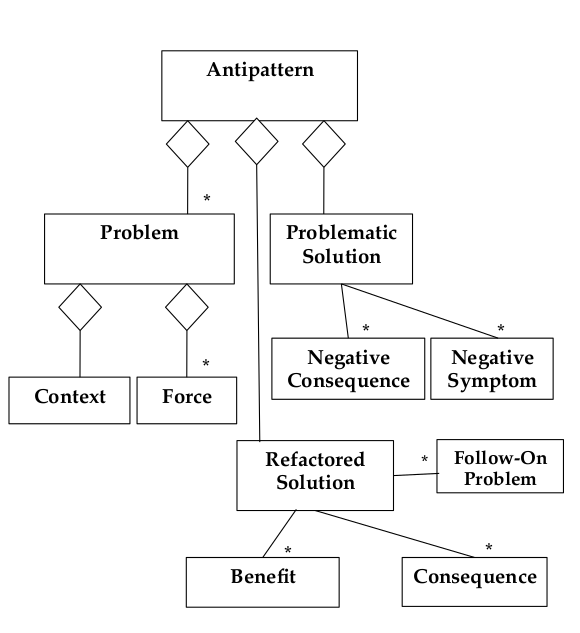
\includegraphics[width=.5\linewidth]{images/antipattern.png}

\textbf{7 Deadly Sins in Software Practice:}
\begin{description}
  \item[Apathy] Not caring about a problem, followed by unwillingness To attempt a solution
  \item[Haste] Solutions based on hasty decisions lead to compromises in software quality
  \item[Narrow-mindedness] The refusal to use solutions that are widely known
  \item[Sloth] Making poor decisions based on "easy" answeres
  \item[Avarice (excessive complexity)] no use of abstractions, excessive modeling of details
  \item[Ignorance] Failure to seek understanding
  \item[Pride] Not invented here: not willing to adopt anything from the outside
\end{description}
\newpage

\subsection{Functional Decomposition}
Functional decomposition describes the decomposition of a system in terms of functions instead of use cases and/or objects (object-oriented decomposition) so that functions are hidden somewhere in the system where nobody might expect them.\\
recommended approach: first decompose in use cases, then in objects.
\begin{description}
  \item[General Form] Everything is a function, lots of files named misc, util,aux,...
  \item[Symptoms and Consequences] \hfill
  \begin{itemize}
    \item Maintainer must understand the whole system to make changes
     \item Code is hard to understand
     \item Code is complex, high coupling between code sections in different files
     \item User interface is often awkward and non-intuitive
  \end{itemize}
  \item[Typical Causes] Wrong trained personal (programmers, designers)

\end{description}
\newpage
